\chapter{UML: Aktivitätsdiagramm}\label{ch:uml_act}
Das Aktivitätsdiagramm zeigt die Abläufe und Prozesse, die in unserem Projekt stattfinden.
In Abbildung ~\ref{fig:act} ist das Aktivitätsdiagramm für unser Projekt dargestellt und zeigt alle Aktivitäten in 
abstrahierter Form zur besseren Verständlichkeit. \\
\newline
Die dargestellte Aktivität dieses Diagramms ist das Gewinnen eines Topfskins durch den Nutzer.
Der Nutzer kann im Menü das Potpack auswählen und es bedingt kaufen.
Falls es keine weiteren verfügbare Skins gibt, wird der Kaufen-Button deaktiviert und es können keine weiteren
Potpacks gekauft werden.
In diesem Abschnitt würde die Aktivität enden und der Nutzer würde das Spiel weiterspielen mit Minispielen und dem 
Halten seine bisherigen und neuen Pflanzen.
Gibt es jedoch noch Skins, die noch nicht im Inventar des Nutzers sind, prüft der Nutzer seinen Münzstand auf die 
benötigte Höhe des Potpacks.\\
Ist der Münzstand ausreichend, wird das Potpack vom Nutzer gekauft und das System wählt zufällig einen Topfskin aus.
Anschließend wird der ausgewählte Topfskin im Potpanel nach der Öffnung des Packs hinzugefügt und aus der Liste der
verfügbaren Skins entfernt. 
Nach der Anzeige des Topfskins durch das System kann der Nutzer das Potpack öffnen und den erhaltenen Topfskin anklicken, 
um ihn seinem Inventar hinzuzufügen.
Hat der Nutzer nicht genug Münzen, können keine Packs geöffnet werden und der Nutzer kann das Spiel weiterspielen.\\

\begin{figure}[h]
    \centering
    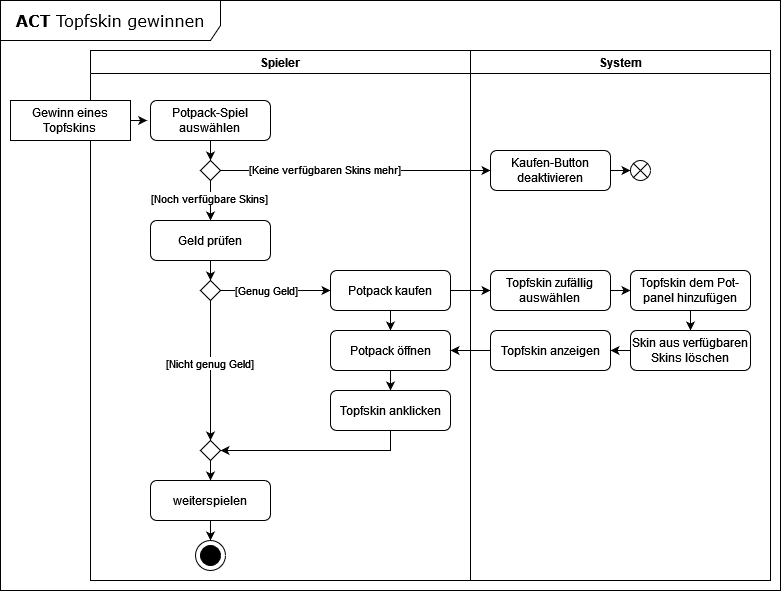
\includegraphics[width=0.8\linewidth]{../bilder/act_potpack}
    \vspace{0.05cm}
    \caption{Aktivitätsdiagramm}
    \label{fig:act}
\end{figure}